
\vspace{-5 mm} 
\begin{IEEEbiography}[{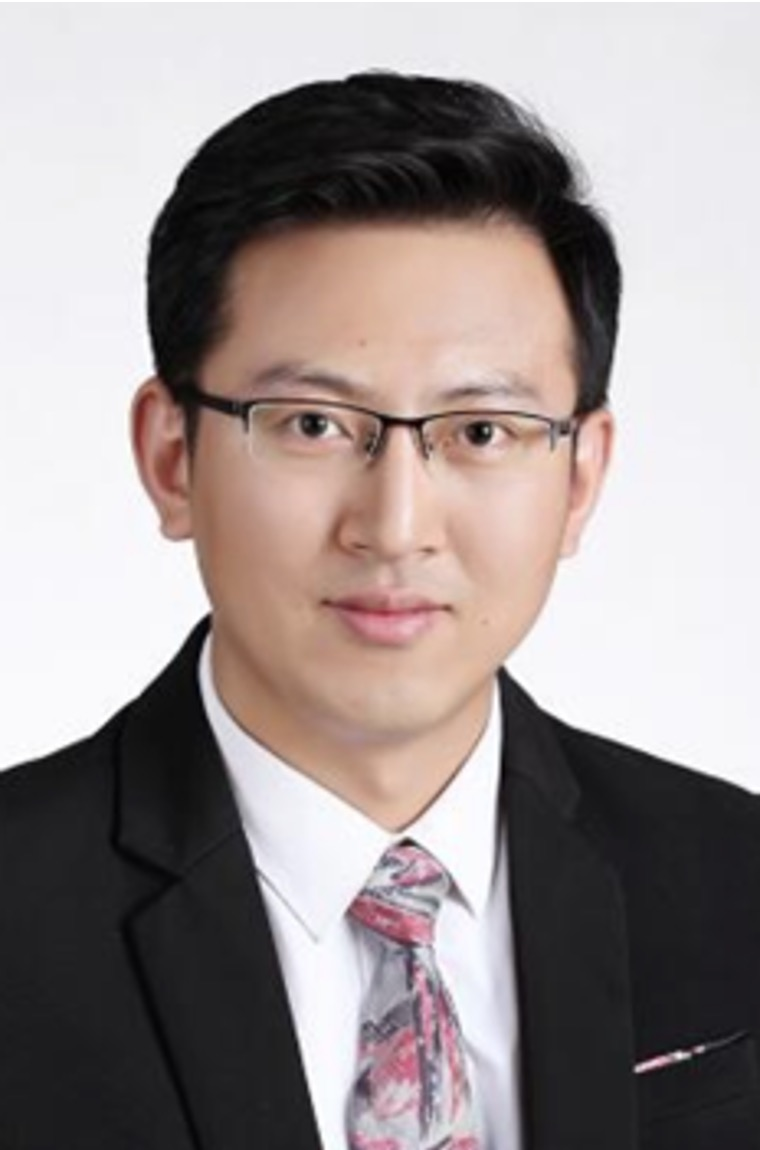
\includegraphics[width=1.02in,keepaspectratio,trim=0 2in 0 0,clip]{biography/liu.jpg}}]{Qingchao Liu }
    received the Ph.D. degree from Southeast University, Nanjing, China, in 2015. He joined the Automotive Engineering Research Institute, Jiangsu University, Zhenjiang, where he is currently working as an Associate Professor. His research interests include Driving behavior analysis, path planning, autonomous vehicle, cooperative adaptive cruise control, traffic flow theory, and intelligent transportation systems. He concurrently serves as a member of the American TRB Artificial Intelligence Subcommittee, a member of the China Society of Automotive Engineers, a member of the China Intelligent Transportation Association, and a senior visiting scholar at Nanyang Technological University in Singapore.
    \end{IEEEbiography}
    
    % if you will not have a photo at all:
    \begin{IEEEbiography}[{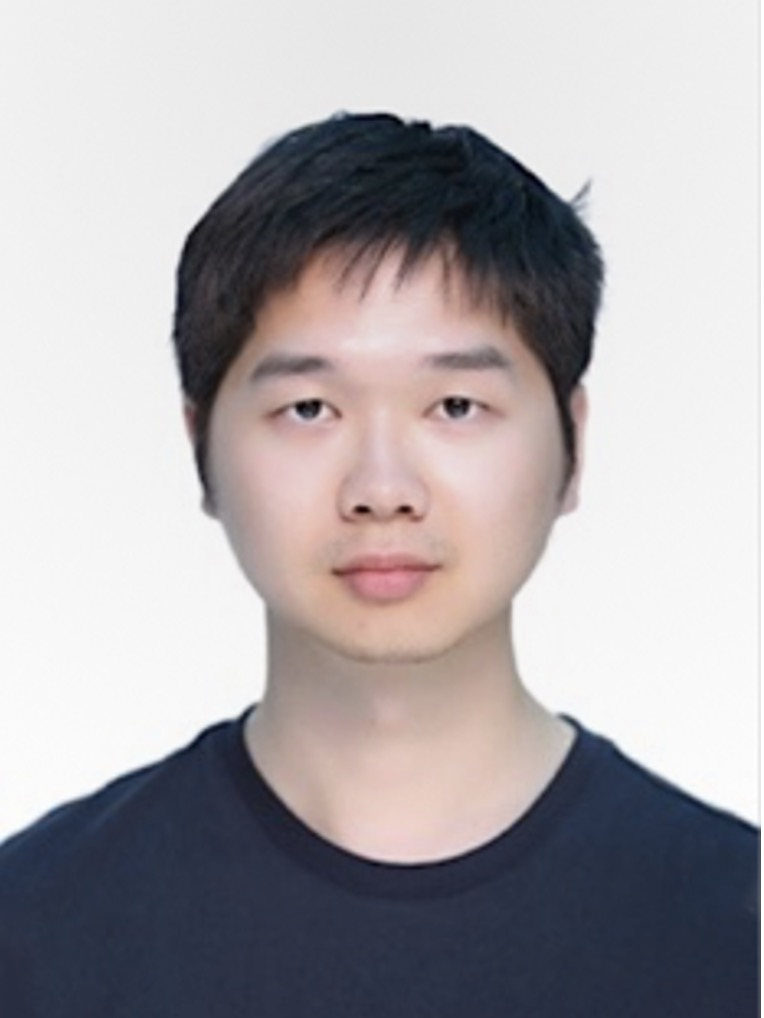
\includegraphics[width=1.02in,keepaspectratio,clip]{biography/gao.jpg}}]{Chengzhi Gao}
    received the bachelor degree in Information and Computing Science from the Anhui Agricultural University in 2022. He is currently pursuing a postgraduate degree in transportation engineering with Jiangsu University, China. His research interests include vehicular platoon control, traffic simulation and intelligent transportation systems. He is currently the deputy leader of the Waliang Lake Ecological Observation Team.
    \end{IEEEbiography}
       % \vspace{-5 mm} 
    \begin{IEEEbiography}[{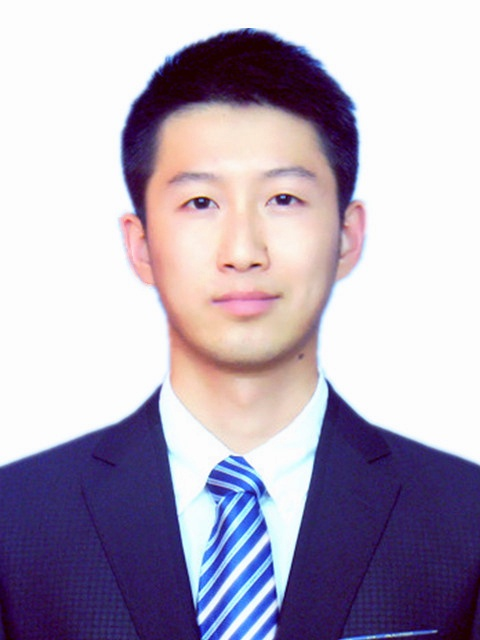
\includegraphics[width=1.02in,keepaspectratio,clip]{biography/hxk.jpg}}]{Xiangkun He}
        (Member, IEEE) is currently a UESTC 100 Young Professor at the University of Electronic Science and Technology of China. Previously, he was a Research Fellow at Nanyang Technological University, Singapore, and served as a Senior Research Scientist at Huawei Noah's Ark Lab from 2019 to 2021. He earned his Ph.D. in 2019 from the School of Vehicle and Mobility at Tsinghua University. He has authored over 50 papers in top-tier journals and conferences, such as TPAMI, TNNLS, TITS, TRC, and Engineering, and holds 8 granted patents. His research interests include reinforcement learning, trustworthy AI, autonomous vehicles, and robotics. He has received many awards and honors, selectively including the Tsinghua University Outstanding Doctoral Dissertation Award in 2019, Best Paper Finalist at IEEE ICMA 2020, Huawei Major Technological Breakthrough Award in 2021, Best Paper Runner-Up Award at CVCI 2022, and Runner-Up in the Intelligent Algorithm Final of the 2022 Alibaba Global Future Vehicle Challenge. He serves as a reviewer for over 50 renowned journals and conferences and was also a member of the award committee for the Autonomous Driving Control Benchmark Challenge at IEEE CDC 2023.
    \end{IEEEbiography} 
    % insert where needed to balance the two columns on the last page with
    % biographies
    %\newpage
    % \vspace{-5 mm} 
    \begin{IEEEbiography}[{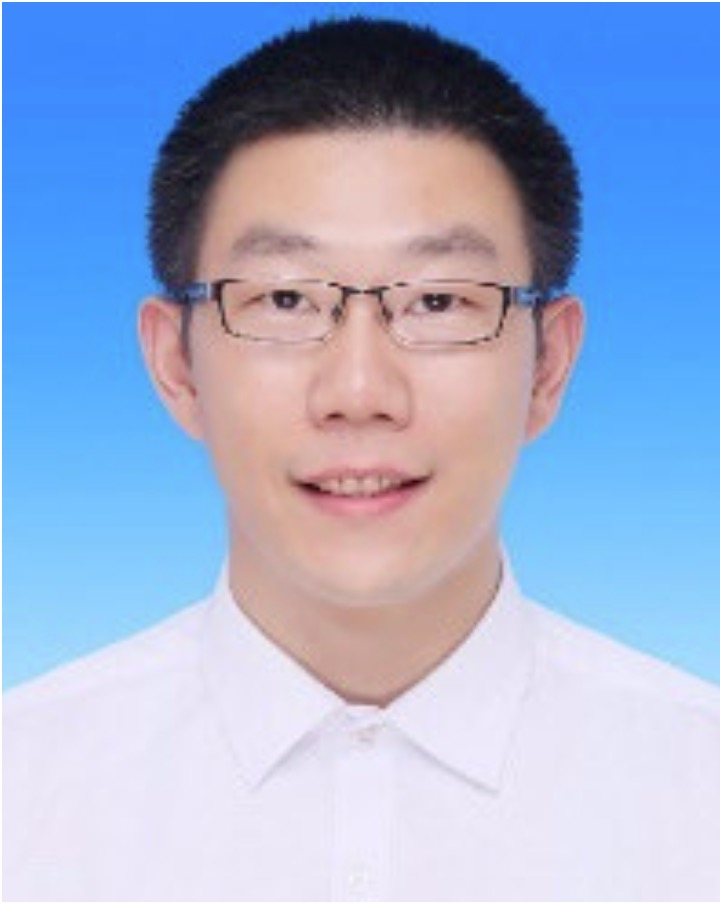
\includegraphics[width=1.02in,keepaspectratio,clip]{biography/wang.jpg}}]{Hai Wang}
        (Senior Member, IEEE) received the B.S., M.S., and Ph.D. degrees from the School of Instrument Science and Engineering, Southeast University, Nanjing, China, respectively. In 2012he joined the School of Automotive and Traffic Engineering at Jiangsu University, where, he is currently working as a Professor. He has authored or coauthored more than 50 papers in the field of machine vision-based environment sensing for intelligent vehicles. His research interests include computer vision, intelligent transportation systems and intelligent vehicles. 
    \end{IEEEbiography}
       
    % \vspace{-5 mm} 
    \begin{IEEEbiography}[{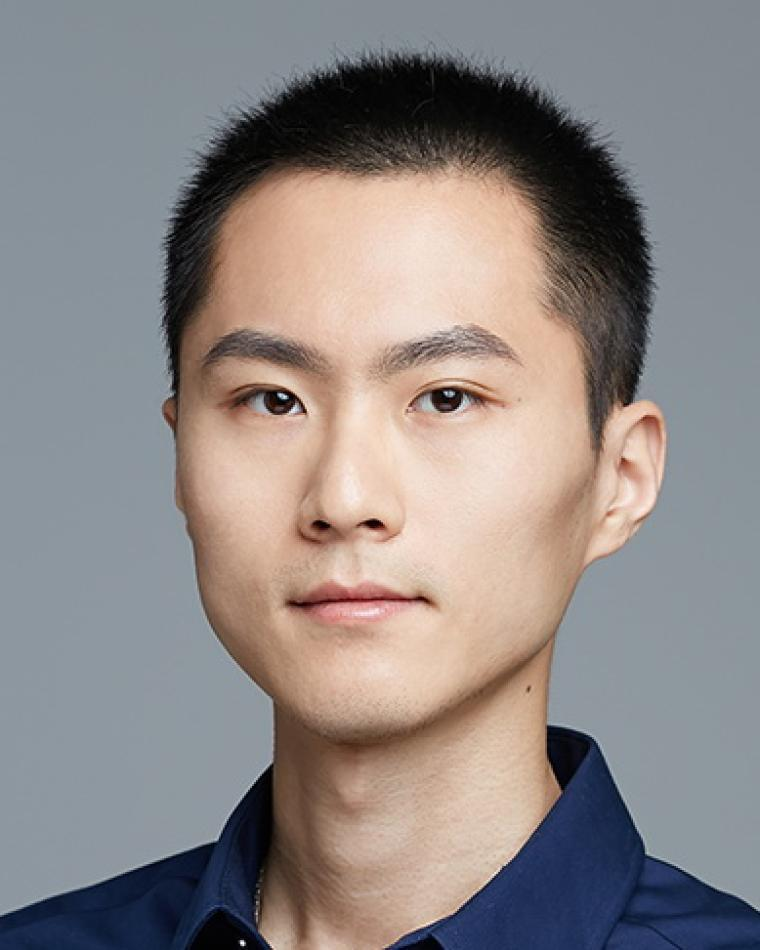
\includegraphics[width=1.02in,keepaspectratio,clip]{biography/lv.png}}]{Chen Lv}
        (Senior Member. IEEE) received the Ph.D. degree from the Department of Automotive Engineering, Tsinghua University China in 2016From 2014 to 2015, he was a joint Ph.D. Researcher with the EECS Department, University of California at Berkeley. He is currently an Assistant Professor with Nanyang Technology University, Singapore. His research interests include cyber-physical systems, hybrid systems, advanced vehicle control, and intelligence, where he has contributed over 90 articles and holds 12 granted Chinese patents. He received the Highly Commended Paper Award of IMechE, U.K., in 2012, the National Fellowship for Doctoral Student in 2013, the NSK Outstanding Mechanical Engineering ward in 2014, the China SAE Outstanding Paper Award. in 2015, the 1st Class Award of China Automotive Industry Scientific and Technological Invention in 2015, the Tsinghua University Outstanding Doctoral Thesis Award in 2016, and the IV2018 Best Workshop/Special Issue Paper Award. He serves as a Guest Editor for IEEE Intelligent Transportation Systems Magazine, IEEE/ASME TRANSACTIONS ON MECHATRONICS, and Applied Energy, and an Associate Editor/Editorial.
    \end{IEEEbiography} 
    % \vspace{-5 mm} 
    \begin{IEEEbiography}[{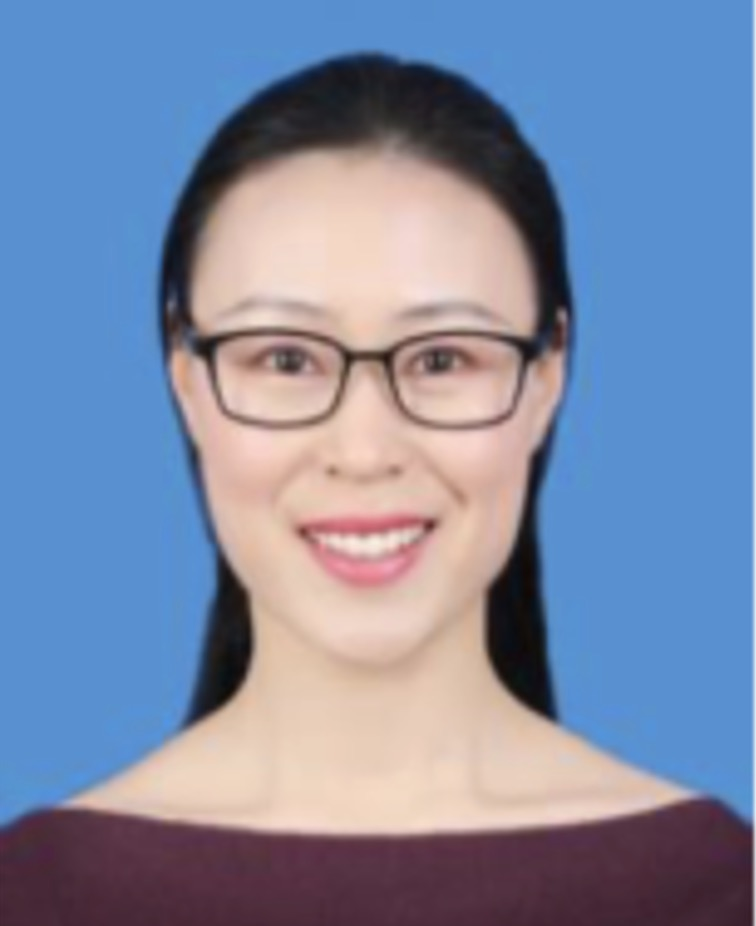
\includegraphics[width=1.02in,keepaspectratio,clip]{biography/cai.jpg}}]{Yingfeng Cai}
        (Senior Member, IEEE) received the B.S., M.S., and Ph.D. degrees from the School of Instrument Science and Engineering, Southeast University, Nanjing. China. In 2013, she joined the Automotive Engineering Research Institute, Jiangsu University, as a Professor. Her research interests include computer vision, intelligent transportation systems. And intelligent automobiles.
    \end{IEEEbiography}
    
    %     % \vspace{-5 mm} 
    \begin{IEEEbiography}[{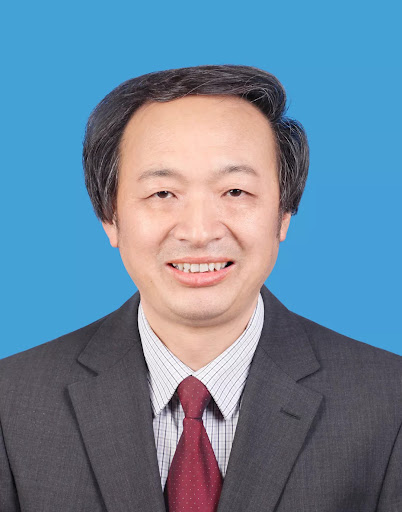
\includegraphics[width=1.02in,keepaspectratio,clip]{biography/chen.jpg}}]{Long Chen}
        received the B.Sc. and Ph.D. degrees in mechanical engineering from Jiangsu University, Zhenjiang, China, in 1982 and 2006, respectively. He is currently a Professor with the Automotive Engineering Research Institute, Jiangsu University Zhenjiang. His research interests include electric vehicles, electric drives, simulation and control of vehicle dynamic performance, vehicle operation, and transport planning.
    \end{IEEEbiography}


    % You can push biographies down or up by placing
    % a \vfill before or after them. The appropriate
    % use of \vfill depends on what kind of text is
    % on the last page and whether or not the columns
    % are being equalized.
    % \vfill

% 使用空白图像作为占位符
% \begin{IEEEbiography}[{\includegraphics[width=1.02in,keepaspectratio]{example-image}}]{Michael Smith}
%     received the Ph.D. degree from the University of California, Los Angeles (UCLA), USA, in 2016. He joined the Mechanical Engineering Department at XYZ University, USA, where he is currently working as an Associate Professor. His research interests include autonomous vehicle technology, human-machine interaction, path planning, traffic optimization, and intelligent transportation systems. He concurrently serves as a member of the SAE Technical Committee on Autonomous Systems, a member of the American Society of Mechanical Engineers, and a visiting scholar at ABC University, UK.
% \end{IEEEbiography}

% % 使用空白图像作为占位符
% \begin{IEEEbiography}[{\includegraphics[width=1.02in,keepaspectratio]{example-image}}]{Alex Johnson}
%     received the bachelor degree in Applied Mathematics from the University of Texas at Austin in 2021. He is currently pursuing a postgraduate degree in transportation systems engineering at XYZ University, USA. His research interests include vehicle platoon optimization, traffic flow simulation, and smart transportation networks. He currently leads the Sustainable Mobility Research Group.
% \end{IEEEbiography}

% % 使用空白图像作为占位符
% \begin{IEEEbiography}[{\includegraphics[width=1.02in,keepaspectratio]{example-image}}]{Robert Brown}
%     (Senior Member, IEEE) received the B.S., M.S., and Ph.D. degrees from the School of Electrical and Computer Engineering at Georgia Institute of Technology, Atlanta, USA. In 2013, he joined the School of Engineering at XYZ University, where he is currently a Professor. He has authored or coauthored over 70 papers in the field of computer vision and sensor systems for intelligent vehicles. His research interests include machine perception, deep learning, and smart transportation infrastructures.
% \end{IEEEbiography}

% % 使用空白图像作为占位符
% \begin{IEEEbiography}[{\includegraphics[width=1.02in,keepaspectratio]{example-image}}]{Emily Davis}
%     (Senior Member, IEEE) received the B.S., M.S., and Ph.D. degrees in Mechanical Engineering from the Massachusetts Institute of Technology (MIT), USA. In 2015, she became a Professor at the Department of Mechanical and Systems Engineering, XYZ University. Her research interests include intelligent transportation systems, autonomous driving technologies, and machine learning applications in mobility.
% \end{IEEEbiography}

% % 使用空白图像作为占位符
% \begin{IEEEbiography}[{\includegraphics[width=1.02in,keepaspectratio]{example-image}}]{James Taylor}
%     received the B.Sc. and Ph.D. degrees in Electrical Engineering from ABC University, UK, in 1985 and 1995, respectively. He is currently a Professor with the Department of Electrical Engineering at XYZ University, USA. His research interests include electric powertrains, control systems for autonomous vehicles, and energy-efficient transportation solutions.
% \end{IEEEbiography}

% % 使用空白图像作为占位符
% \begin{IEEEbiography}[{\includegraphics[width=1.02in,keepaspectratio]{example-image}}]{Sophia Wilson}
%     (Senior Member, IEEE) received the Ph.D. degree in Mechanical Engineering from the University of Cambridge, UK, in 2017. From 2016 to 2017, she was a visiting researcher at the University of California, Berkeley. She is currently an Assistant Professor with the Department of Engineering at ABC University, Singapore. Her research interests include cyber-physical systems, energy-efficient transportation, intelligent vehicle control systems, and cooperative driving technologies. She has authored over 80 articles and holds 10 international patents. She has received a number of awards, including the Excellence in Research Award from the Society of Mechanical Engineers in 2020 and the Best Paper Award at the International IEEE Transportation Conference in 2019. She serves as an Associate Editor for IEEE Transactions on Intelligent Vehicles and several other international journals.
% \end{IEEEbiography}